\documentclass[t,usenames,dvipsnames]{beamer}
\usetheme{Copenhagen}
\setbeamertemplate{headline}{} % remove toc from headers
\beamertemplatenavigationsymbolsempty

\usepackage{amsmath, xcolor, tikz, pgfplots}

\pgfplotsset{compat = 1.16}
\usetikzlibrary{arrows.meta, calc, decorations.pathreplacing}
\pgfplotsset{every axis/.append style = {axis lines = middle}}
\pgfplotsset{every tick label/.append style={font=\scriptsize}}
\everymath{\displaystyle}

\title{Absolute Value Inequalities}
\author{}
\date{}

\AtBeginSection[]
{
  \begin{frame}
    \frametitle{Objectives}
    \tableofcontents[currentsection]
  \end{frame}
}

\begin{document}

\begin{frame}
    \maketitle
\end{frame}

\section{Solve absolute value equations}



\begin{frame}{Solving Absolute Value Equations}
When solving absolute value equations, you will typically get 2 distinct answers to your equation.   \newline\\ \pause

Try to get the absolute value expression alone and break into 2 cases.
\end{frame}

\begin{frame}{Example 1}
Solve $|3x-1| = 6$
\begin{align*}
    \onslide<2->{3x-1&=6 & 3x-1&=-6} \\[8pt]
    \onslide<3->{3x&=7 & 3x&=-5} \\[8pt]
    \onslide<4->{x&=\frac{7}{3} & x&=-\frac{5}{3}}
\end{align*}
\end{frame}

\section{Solve absolute value inequalities}

\begin{frame}{General Method of Solving Inequalities}
To solve inequalities, we can solve their equation equivalent. \newline\\

Then we can use \alert{test values} to determine which values make the original inequality true.
\end{frame}

\begin{frame}{Example 2}
Solve each. \newline\\
(a) \quad $|x-1|\geq 3$
\begin{align*}
    \onslide<2->{x-1&=3 & x-1&=-3} \\[6pt]
    \onslide<3->{x&=4 & x&=-2} 
\end{align*}
\begin{center}
\onslide<4->{
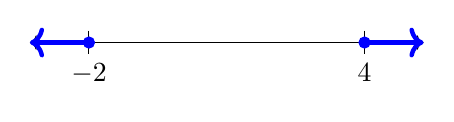
\begin{tikzpicture}
\draw[<->] (-2.5,0) -- (2.5,0);
\draw (-1.75,0.15) -- (-1.75,-0.15) node [below] {$-2$};
\draw (1.75,0.15) -- (1.75,-0.15) node [below] {$4$};
\onslide<5->{
\draw[color=blue,fill=blue] (-1.75,0) circle [radius = 2pt];
\draw[color=blue,fill=blue] (1.75,0) circle [radius=2pt];}
\onslide<6->{
\draw[color=blue, ultra thick, ->] (-1.75,0) -- (-2.5,0);
\draw[color=blue, ultra thick, ->] (1.75,0) -- (2.5,0);}
\end{tikzpicture}}
\onslide<7->{\[(-\infty, -2] \cup [4, \infty) \]}
\end{center}
\end{frame}

\begin{frame}{Graphical Interpretation of Example 2a}
(a) \quad $|x-1|\geq 3$ 
\[(-\infty, -2] \cup [4, \infty) \]
\begin{center}
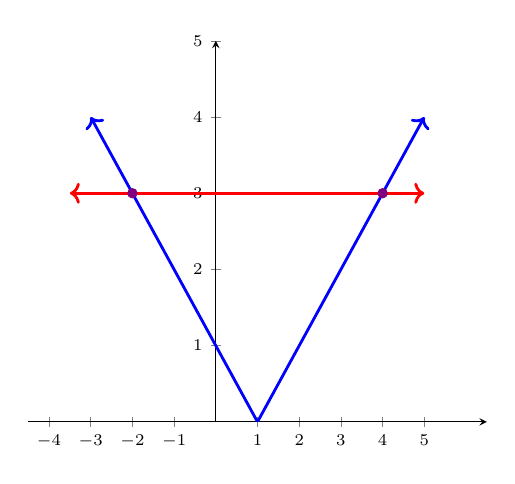
\begin{tikzpicture}[scale=0.85]
\begin{axis}[
xmin = -4.5, xmax = 6.5,
ymin = 0, ymax = 5,
xtick = {-4,-3,...,5},
ytick = {0,1,...,5}
]
\addplot[color=blue, very thick, <->, domain=-3:5] {abs(x-1)};
\addplot[color=red, very thick, <->, domain=-3.5:5] {3};
\addplot[color=violet, mark=*, only marks] coordinates {(-2,3) (4,3)};
\end{axis}
\end{tikzpicture}
\end{center}
\end{frame}

\begin{frame}{Graphical Interpretation of Solutions to Inequalities}
Given two functions $f(x)$ and $g(x)$:  \newline\\  \pause
\begin{itemize}
    \item<+-> $f(x) > g(x)$: Where $f(x)$ is above $g(x)$ \newline\\
    \item<+-> $f(x) \geq g(x)$: Where $f(x)$ is at or above $g(x)$ \newline\\
    \item<+-> $f(x) < g(x)$: Where $f(x)$ is below $g(x)$ \newline\\
    \item<+-> $f(x) \leq g(x)$: Where $f(x)$ is at or below $g(x)$
\end{itemize}
\end{frame}

\begin{frame}{Example 2}
(b) \quad $4-3|2x+1| > -2$
\begin{align*}
    \onslide<2->{4-3|2x+1| &= -2} \\[6pt]
    \onslide<3->{-3|2x+1| &= -6} \\[6pt]
    \onslide<4->{|2x+1| &= 2}
\end{align*}
\begin{align*}
    \onslide<5->{2x+1 &= 2 & 2x+1&=-2} \\[6pt]
    \onslide<6->{x&=\frac{1}{2} & x&= -\frac{3}{2}}
\end{align*}
\end{frame}

\begin{frame}{Example 2}
(b) \quad $4-3|2x+1| > -2$
\[x = \frac{1}{2} \quad x = -\frac{3}{2} \]
\vspace{11pt}
\begin{center}
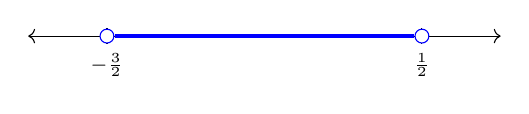
\begin{tikzpicture}
\draw[<->] (-3,0) -- (3,0);
\draw (-2,0.1) -- (-2,-0.1) node [below] {\scriptsize $-\frac{3}{2}$};
\draw (2,0.1) -- (2,-0.1) node [below] {\scriptsize $\frac{1}{2}$};
\onslide<2->{
\draw[color=blue,fill=white] (-2,0) circle [radius=2.5pt];
\draw[color=blue,fill=white] (2,0) circle [radius=2.5pt];}
\onslide<3->{\draw[ultra thick, color=blue] (-2+0.1,0) -- (2-0.1,0);}
\end{tikzpicture}
\onslide<4->{\[\left(-\frac{3}{2},\frac{1}{2}\right)\]}
\end{center}
\end{frame}

\begin{frame}{Example 2}
(b) \quad $4-3|2x+1| > -2$  \newline\\  
\begin{center}
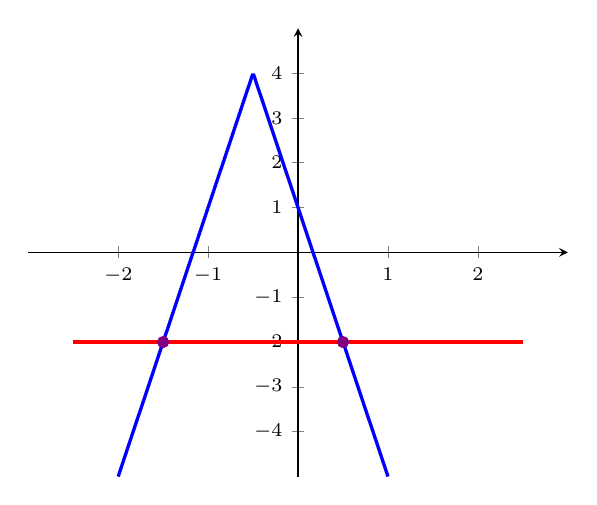
\begin{tikzpicture}
\begin{axis}[
xmin = -3, xmax = 3,
ymin = -5, ymax = 5,
xtick = {-2,-1,0,1,2},
ytick = {-4,-3,...,4}
]
\addplot[color=blue, very thick, samples=200, smooth, domain=-2:1]{4-3*abs(2*x+1)};
\addplot[color=red, very thick, domain=-2.5:2.5] {-2};
\addplot[color=violet, mark=*, only marks] coordinates {(-1.5,-2) (0.5,-2)};
\end{axis}
\end{tikzpicture}
\end{center}
\end{frame}

\begin{frame}{Example 2}
(c) \quad $2 < |x-1| \leq 5$
\onslide<2->{\[2 < |x-1| \quad \text{and} \quad |x-1| \leq 5 \]}
\begin{align*}
    \onslide<3->{x-1&=-2 & x-1&=2 & x-1&=5 & x-1&=-5} \\
    \onslide<4->{x&=-1 & x&=3 & x&=6 & x&= -4} \\
\end{align*}
\begin{center}
\onslide<5->{
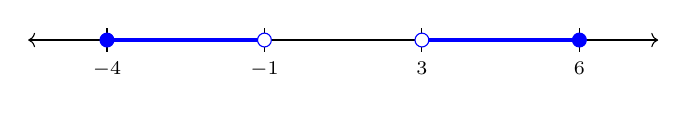
\begin{tikzpicture}
\draw[<->] (-4,0) -- (4,0);
\draw (-3,0.15) -- (-3,-0.15) node [below] {\scriptsize $-4$};
\draw (-1,0.15) -- (-1,-0.15) node [below] {\scriptsize $-1$};
\draw (1,0.15) -- (1,-0.15) node [below] {\scriptsize $3$};
\draw (3,0.15) -- (3,-0.15) node [below] {\scriptsize $6$};
\onslide<6->{
\draw[color=blue,ultra thick] (-3,0)--(-1,0);
\draw[color=blue,ultra thick] (1,0) -- (3,0);
\draw[color=blue,fill=blue] (-3,0) circle [radius=2.5pt];
\draw[color=blue,fill=blue] (3,0) circle [radius=2.5pt];
\draw[color=blue,fill=white] (-1,0) circle [radius=2.5pt];
\draw[color=blue,fill=white] (1,0) circle [radius=2.5pt];
}
\end{tikzpicture}}
\end{center}
\onslide<7->{\[[-4,-1) \cup (3,6]\]}
\end{frame}

\begin{frame}{Example 2}
(c) \quad $2 < |x-1| \leq 5$    \newline\\
\begin{center}
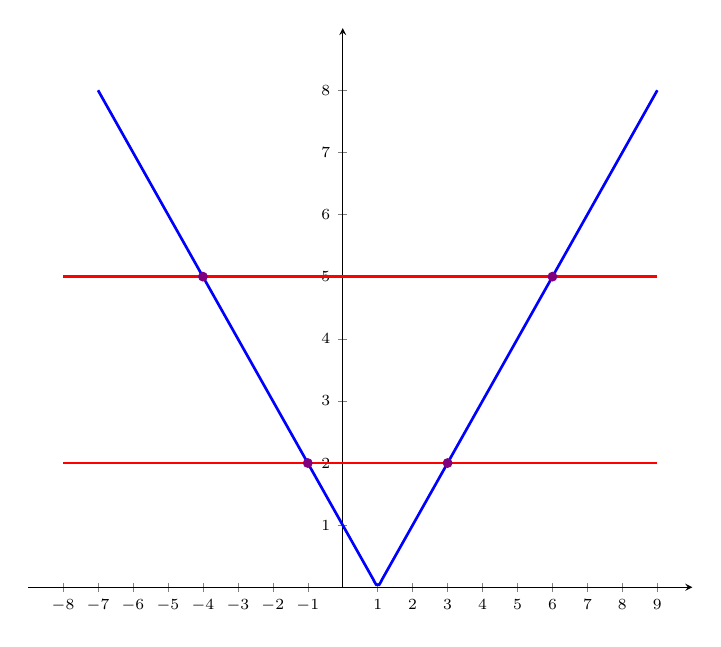
\begin{tikzpicture}[scale=0.8]
\begin{axis}[
xmin = -9, xmax = 10,
ymin = 0, ymax = 9,
xtick = {-8,-7,...,9},
ytick = {1,2,...,8},
width = \textwidth
]
\addplot[blue, very thick, samples=200, smooth, domain=-7:9]{abs(x-1)};
\addplot[red, very thick, domain=-8:9] {5};
\addplot[red, very thick, domain=-8:9] {2};
\addplot[violet, mark=*, only marks] coordinates {(-4,5) (-1,2) (3,2) (6,5)};
\end{axis}
\end{tikzpicture}
\end{center}
\end{frame}

\begin{frame}{Example 2}
(d) \quad $|x+1|\geq\frac{x+4}{2}$
\begin{align*}
    \onslide<2->{x+1&=\frac{x+4}{2} & x+1&=-\frac{x+4}{2}} \\[8pt]
    \onslide<3->{2x+2&=x+4 & -2x-2&=x+4} \\[8pt]
    \onslide<4->{x&=2 & x&=-2}
\end{align*}
\begin{center}
\onslide<5->{
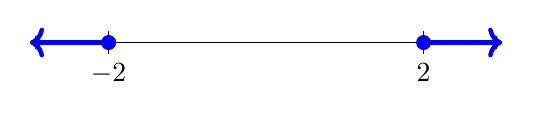
\begin{tikzpicture}
\draw[<->] (-3,0) -- (3,0);
\draw (-2,0.15) -- (-2,-0.15) node [below] {$-2$};
\draw (2,0.15) -- (2,-0.15) node [below] {$2$};
\onslide<6->{\draw[color=blue,fill=blue] (-2,0) circle [radius=2.5pt];
\draw[color=blue,fill=blue] (2,0) circle [radius=2.5pt];
\draw[color=blue, ultra thick, ->] (-2,0) -- (-3,0);
\draw[color=blue, ultra thick, ->] (2,0) -- (3,0);}
\end{tikzpicture}}
\end{center}
\onslide<7->{\[(-\infty, -2] \cup [2, \infty)\]}
\end{frame}

\begin{frame}{Example 2}
(d) \quad $|x+1|\geq\frac{x+4}{2}$  \newline\\
\begin{center}
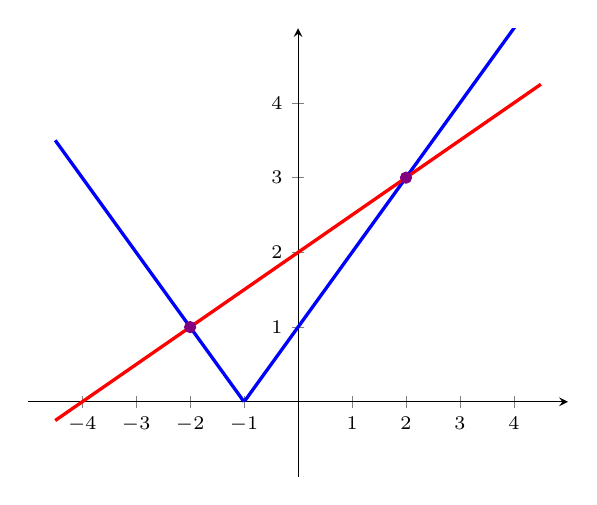
\begin{tikzpicture}
\begin{axis}[
xmin=-5, xmax=5,
ymin=-1, ymax=5,
xtick={-4,-3,...,4},
ytick={1,2,3,4}
]
\addplot[color=blue, very thick, domain=-4.5:4.5, smooth, samples=200] {abs(x+1)};
\addplot[color=red, very thick, domain=-4.5:4.5] {0.5*x+2};
\addplot[color=violet, mark=*, only marks] coordinates {(-2,1) (2,3)};
\end{axis}
\end{tikzpicture}
\end{center}
\end{frame}

\end{document}
